    \documentclass[conference]{IEEEtran}

    \usepackage{amsmath,amssymb,amsfonts}
    \usepackage{graphicx}
    \usepackage{cite}
    \usepackage{algorithm}
    \usepackage{algorithmic}
    \usepackage{array}
    \usepackage{booktabs}

    \title{Fault-Tolerant and Load-Balanced IIoT Edge–Fog Architecture over Multiple Kubernetes Clusters}

    \author{
    \IEEEauthorblockN{
    Benyapa Tawunwoot\IEEEauthorrefmark{1},
    Proud Pitugkittikul\IEEEauthorrefmark{2},
    Ramona Bhuthontharaj\IEEEauthorrefmark{3},\\
    Nang Yein Mo Hsai\IEEEauthorrefmark{4},
    Somchart Fugkeaw\IEEEauthorrefmark{5}
    }
    \IEEEauthorblockA{
    School of Information, Computer, and Communication Technology (ICT)\\
    Sirindhorn International Institute of Technology (SIIT), Thammasat University, Thailand\\
    Email:
    \IEEEauthorrefmark{1}6622770509@g.siit.tu.ac.th,
    \IEEEauthorrefmark{2}6622770665@g.siit.tu.ac.th,
    \IEEEauthorrefmark{3}6622782140@g.siit.tu.ac.th,\\
    \IEEEauthorrefmark{4}m6822041015@g.siit.tu.ac.th,
    \IEEEauthorrefmark{5}somchart@siit.tu.ac.th
    }
    }


    \begin{document}

    \maketitle

    \begin{abstract}
    This paper proposes a fault-tolerant and load-balanced Industrial Internet of Things (IIoT) edge--fog architecture deployed over multiple Kubernetes clusters for secure and low-latency data processing. The framework combines fog-scoped sensor AES keys, trusted execution environment (TEE)-enforced key transformation, Paillier slot aggregation, gossip-based load balancing, sensor-side ACK redirects, and cloud-layer ciphertext-policy attribute-based encryption (CP-ABE). To address workload dynamics and fog failures in heterogeneous fog environments, fog nodes exchange status through a decentralized gossip protocol and check the most recent workload table on every incoming sensor reading. Overload is handled through KMM-provisioned enclave delegation without sensor retransmission, while ACK timeout allows sensors to redirect encrypted readings after direct fog silence and notify the KMM for delegated key provisioning. Vacated aggregation slots are filled with Paillier encryptions of zero when the original fog node remains alive, and the key management module combines one aggregate ciphertext per fog node at each 500~ms window close. Overall, the proposed scheme jointly supports fog-scoped key isolation, adaptive per-reading delegation, bounded-loss ACK-based recovery, storage-efficient aggregation, and resilient fog operation for time-sensitive industrial monitoring and control applications.
    \end{abstract}

    \begin{IEEEkeywords}
    Industrial Internet of Things, Edge--fog computing, Fault tolerance, Load balancing, Trusted execution environment, Paillier encryption, Kubernetes
    \end{IEEEkeywords}

    \section{Introduction}
    The Industrial Internet of Things (IIoT) has become a foundational 
    pillar of Industry~4.0, enabling continuous monitoring, predictive 
    maintenance, and automated control across large-scale industrial 
    environments~\cite{tange2020}. Numerous sensors and control devices 
    generate time-sensitive data streams that impose strict requirements 
    on latency, reliability, and security. For example, vibration sensors 
    on rotating machinery produce hundreds of measurements per second, 
    while safety monitoring systems in chemical plants must detect 
    abnormal conditions in real time to prevent hazardous 
    incidents~\cite{farooq2023}.

    Centralized cloud architectures struggle to satisfy these latency 
    requirements due to the long communication path between sensors and 
    remote data centers. Edge and fog computing have emerged as the 
    dominant solution, moving computation closer to data 
    sources~\cite{jin2024}. In an edge--fog architecture, edge gateways 
    perform initial preprocessing near IIoT devices while fog nodes 
    provide intermediate aggregation and analytics before forwarding 
    results to the cloud, significantly reducing latency and bandwidth 
    overhead.

    Despite these advantages, fog-based IIoT deployments face three 
    critical challenges. First, heterogeneous fog nodes subject to static 
    workload assignment create resource imbalance, where weaker nodes 
    become overloaded while stronger nodes remain 
    underutilized~\cite{kashani2023}. Second fault tolerance mechanisms in fog environments introduce extra computational and storage overhead, which affects performance in resource-constrained settings~\cite{chen2024lb}. Third, many 
    existing systems require fog nodes to decrypt sensor data before 
    performing aggregation, violating the zero-trust assumption of modern 
    distributed infrastructures and exposing sensitive industrial data at 
    the fog layer~\cite{mirani2022}.



    Prior work addresses each challenge independently but creates new 
    tradeoffs when combined. Global shared AES key schemes allow 
    efficient key management but mean that a single compromised fog node 
    exposes all sensor data across the entire deployment. Per-reading 
    Paillier encryption~\cite{peng2022} preserves fog-layer privacy but 
    transmits $n$ ciphertexts per window to the cloud, causing storage 
    overhead that grows linearly with sensor count. Replication-based 
    fault tolerance ensures service continuity but duplicates 
    already-large ciphertexts, amplifying the storage problem. No 
    existing work eliminates all three tradeoffs within a single unified 
    architecture.

    Beyond the fog layer, most existing IIoT architectures deploy 
    analytics services within a single Kubernetes cluster, which 
    remains vulnerable to cluster-level failures that can interrupt 
    all services simultaneously~\cite{burns2016}. Such failures are 
    particularly critical in industrial environments requiring 
    continuous operation, such as predictive maintenance and power 
    grid monitoring~\cite{burhan2023}.

    To address these limitations, this paper proposes a fault-tolerant 
    and load-balanced IIoT edge--fog architecture deployed over multiple 
    Kubernetes clusters. The proposed framework integrates fog-scoped AES 
    key isolation enforced by Intel SGX trusted execution 
    environments~\cite{costan2016}, Paillier homomorphic slot 
    aggregation~\cite{paillier1999}, gossip-based adaptive load 
    balancing, and CP-ABE cloud-layer access control~\cite{penuelasmsa2024}, 
    providing end-to-end data confidentiality without exposing plaintext 
    at any intermediate processing stage.

    \section{Related Work}
    This section reviews existing literature relevant to the proposed secure IIoT fog computing system. The related work is organized into two main areas: (1) load balancing and fault tolerance in fog computing environments, and (2) encryption schemes and trusted execution mechanisms for IIoT data security, including symmetric encryption, trusted execution environments, homomorphic encryption, attribute-based encryption, and hybrid cryptographic approaches.

    \subsection{Encryption Schemes for IIoT and Fog Computing}
    Securing data in IIoT and fog architectures requires protecting sensor
    measurements across untrusted intermediate nodes while ensuring confidentiality,integrity, and fine-grained access control. This subsection surveys the cryptographic and hardware-enforced building blocks most relevant to this problem: AES-based sensor encryption, trusted execution environments for secure key transformation and delegation, homomorphic encryption for privacy-preserving aggregation, and ciphertext-policy attribute-based encryption for cloud access control. Each area is examined with attention to
    the limitations of existing proposals and the open problems that motivate the
    contributions of this paper.

    \subsubsection{Symmetric Encryption (AES) for Lightweight Sensor Security}
    AES remains the dominant symmetric cipher in IIoT sensor deployments owing to its hardware acceleration support, strong provable security, and NIST standardization~\cite{nist_aes}. Neshenko et al.~\cite{neshenko2019} survey IIoT vulnerability classes and conclude that sensor-layer symmetric encryption is a necessary first line of defense, as it prevents passive eavesdropping on wireless channels without imposing public-key overhead on resource-constrained devices. Simplicio et al.~\cite{simplicio} demonstrate that AES-128 in CTR mode achieves adequate throughput on Cortex-M0 class processors while keeping energy consumption within the budget of battery-operated sensors, and Liuet al.~\cite{liu2021} show that lightweight AES variants can be integrated with fog offloading pipelines at sub-millisecond encryption latency per packet. More recent work has examined AES in the context of evolving lightweight cryptography standards. Sevin and Mohammed~\cite{sevin2023} conduct a comparative software implementation survey of lightweight block ciphers for constrained IoT devices and find that AES-128 continues to provide the best security-to-performance ratio on devices equipped with hardware acceleration,while alternatives such as ASCON may be preferable when no hardware accelerator is available. Amrita et al.~\cite{amrita2024} similarly conclude that AES remains appropriate for fog-adjacent gateway nodes but caution that devices below the Cortex-M3 class require algorithm-level optimizations to meet latency targets in high-frequency sensor deployments. A recent comprehensive survey on lightweight cryptographic mechanisms specifically for IIoT~\cite{iiot_lwc2025} identifies AES-128 as the recommended minimum-security baseline consistent with ISO/IEC 29192, yet also highlights that the majority of existing schemes apply AES only at the sensor layer without addressing how the resulting ciphertext should be processed, delegated, or re-encrypted at intermediate fog nodes. This observation underscores the need for multi-layer architectures that extend beyond single-point symmetric encryption.

    \subsubsection{Trusted Execution Environments for Secure Delegation}

    Trusted execution environments (TEEs), such as Intel SGX, provide hardware-isolated execution contexts whose memory is protected from the host operating system and other privileged software. In fog computing environments, this property enables a different delegation model from proxy re-encryption: instead of asking a semi-trusted proxy to transform ciphertexts across incompatible schemes, the enclave can hold sealed key material, decrypt and re-encrypt data internally, and prove the integrity of the enclave code through remote attestation before keys are provisioned.

    TEE-based designs are particularly relevant when a pipeline must bridge cryptographic domains. AES ciphertexts, Paillier ciphertexts, and AES storage ciphertexts are not interchangeable objects under a single re-encryption operation. A TEE therefore provides a practical enforcement boundary for operations that require plaintext or secret keys temporarily inside the fog node while keeping those values inaccessible to the honest-but-curious host OS. The remaining open problem is how to combine this hardware-backed key transformation with adaptive workload delegation so that overload and failure recovery do not require constrained sensors to generate fresh delegation keys or retransmit measurements.

    \subsubsection{Paillier Homomorphic Encryption for Privacy-Preserving Fog
    Aggregation}

    Homomorphic encryption, fully formalized by Gentry~\cite{gentry2009} and made
    practically efficient in leveled form by the BFV~\cite{bfv2012} and
    CKKS~\cite{ckks2017} schemes, allows computations to be performed directly on
    ciphertexts without decryption. Acar et al.~\cite{acar2018} survey practical HE
    constructions and conclude that leveled schemes such as BFV are well-suited for
    fog aggregation workloads where the multiplicative depth required by common
    aggregation functions (sum, weighted average, threshold count) is low. Froelicher
    et al.~\cite{froelicher2021} propose a distributed HE aggregation protocol for
    multi-party analysis and demonstrate that HE-based aggregation across
    geographically distributed nodes is feasible at scale. Lu et
    al.~\cite{lu2017} apply CKKS-based HE to fog-cloud pipelines for IoT sensor
    aggregation and report latency compatible with one-second reporting intervals.

    Recent work has further validated HE for IIoT aggregation while exposing
    important limitations. Wang et al.~\cite{wang2024smpc} address secure real-time
    data aggregation in IIoT using secret sharing combined with partially
    homomorphic encryption and note that fully homomorphic constructions impose
    impractical overhead for dense real-time pipelines, while partial schemes
    restrict the types of aggregation that can be supported to a single arithmetic
    operation. Abbas et al.~\cite{abbas2024bmda} propose a blockchain-based
    multifunctional aggregation method for fog-IoT using Paillier homomorphic
    encryption and demonstrate that ciphertext expansion and key management overhead
    remain practical challenges at scale, particularly when aggregated ciphertexts
    must be stored and later queried in a cloud environment. Zhang et
    al.~\cite{zhang2022mohe} provide a systematic method for BFV parameter
    selection based on target multiplicative depth and security level, informing
    the tradeoff between computational precision and ciphertext expansion that must
    be resolved in heterogeneous sensor deployments.

    A recurring gap in this body of work is the absence of a domain conversion
    mechanism that decouples the HE computation domain from a more compact storage
    domain. When aggregated HE ciphertexts must be stored in the cloud, the
    substantial ciphertext expansion inherent to HE introduces storage overhead
    and forces cloud services to hold HE private keys, unnecessarily widening the
    trust boundary. Existing schemes do not address how this domain gap can be
    bridged efficiently while preserving the honest-but-curious cloud adversary
    assumption.

    In this work, the homomorphic layer is instantiated with Paillier encryption rather than a generic HE scheme. Paillier directly supports additive aggregation, mean computation after decryption, and weighted sums through scalar multiplication, which covers the target class of fixed-window IIoT aggregation workloads. Operations requiring ciphertext multiplication or comparison, such as variance, maximum, minimum, and threshold counting, are outside the Paillier-only scope.

    \subsubsection{Ciphertext-Policy Attribute-Based Encryption (CP-ABE) for
    Fine-Grained Access Control}

    Attribute-based encryption was introduced by Sahai and Waters~\cite{sahai2005}
    and extended to the ciphertext-policy setting by Bethencourt, Sahai, and
    Waters~\cite{bethencourt2007}, enabling data-centric access policies to be
    embedded directly in ciphertexts. Li et al.~\cite{li2013} demonstrate CP-ABE
    access control for smart grid data in the cloud and show that the scheme scales
    as the number of attribute authorities and authorized consumers grows, making it
    suitable for multi-tenant deployments. Ibraimi et al.~\cite{ibraimi2009} propose
    a mediated CP-ABE construction supporting attribute revocation without
    re-encryption of stored ciphertexts, an important practical requirement when
    service accounts are dynamically decommissioned. Yang et al.~\cite{yang2013}
    integrate CP-ABE with fog computing to enforce access control at the fog tier
    before data reaches the cloud, thereby reducing the exposure window for
    sensitive IIoT data.

    More recent work has targeted computational efficiency and multi-authority
    scenarios. Qu et al.~\cite{qu2024cpabe} propose a pairing-free CP-ABE scheme
    for IoT based on elliptic curve scalar multiplication with multi-authority key
    management and verifiable outsourced decryption; this significantly reduces
    decryption cost on constrained devices but does not address decryption by
    containerized analytics services in a multi-cluster deployment environment. Li
    et al.~\cite{li2025fhac} present an efficient fine-grained access control
    scheme with fully hidden policies for cloud-enabled IoT using bloom filters to
    match attributes without revealing the policy structure; however, the scheme
    assumes a single-authority trust model and does not integrate with HE-based fog
    aggregation pipelines. Pe\~{n}uelas-Angulo et al.~\cite{penuelas2024} propose a
    revocable multi-authority ABE scheme for fog-enabled IoT that outsources partial
    decryption to fog nodes to reduce end-device decryption latency; this design
    introduces fog-side decryption, which conflicts with honest-but-curious threat
    models requiring fog nodes to remain oblivious to plaintext. Das and
    Namasudra~\cite{das2023} propose a multi-authority CP-ABE access control model
    for IoT-enabled healthcare infrastructure and show that distributing attribute
    management across authorities improves resilience, yet rely on a centralized
    key distribution server that constitutes a single point of failure in industrial
    deployments.

    Despite these advances, existing CP-ABE schemes for fog and cloud environments
    are generally evaluated in isolation from HE aggregation pipelines or
    Paillier slot-aggregation and TEE-assisted load balancing mechanisms. The integration of fine-grained access
    control with prior cryptographic stages remains an open design problem for
    IIoT architectures.

    \subsubsection{Hybrid Cryptographic Schemes for IIoT}

    Practical IIoT deployments increasingly combine multiple cryptographic
    primitives into hybrid pipelines that balance security strength with
    performance constraints. Qin et al.~\cite{qin2022} survey delegation schemes for
    cloud data sharing and highlight the efficiency of hybrid AES-ABE patterns in
    which AES encrypts bulk data while ABE protects the symmetric key. Fu et
    al.~\cite{fu2015} demonstrate that three-layer hybrid pipelines can remain
    computationally feasible on ARM Cortex-A class fog hardware. Raisaro et
    al.~\cite{raisaro2017} present a four-layer pipeline combining symmetric source
    encryption, homomorphic aggregation, domain conversion, and ABE-based access
    control, providing empirical evidence that the combined pipeline latency is
    compatible with real-time reporting requirements.

    Recent hybrid proposals have continued to expand this design space. Rani
    et al.~\cite{rani2024} propose a hybrid AES-ECC framework for fog-based smart
    grid IoT that demonstrates layered encryption can improve privacy while
    maintaining acceptable latency; however, the scheme does not incorporate homomorphic encryption for
    computation over ciphertexts and provides no mechanism for encrypted workload
    reassignment. A 2025 adaptive fog encryption study~\cite{adaptive2025} employs
    machine learning to dynamically select among symmetric and hybrid cryptographic
    schemes based on data sensitivity and network context, improving overall
    pipeline efficiency; this approach, however, does not address scenarios in which
    fog nodes become overloaded or fail during aggregation.

    Despite the progress surveyed above, no existing hybrid IIoT pipeline
    simultaneously satisfies all four of the following properties in a fog-cloud
    context: (i) fog-scoped lightweight AES encryption at the sensor layer, (ii) KMM-provisioned
    attested enclave delegation supporting both load balancing and fault tolerance
    without requiring sensor retransmission during overload handling and with ACK-timeout retransmission for direct failed-node recovery, (iii) Paillier slot-grouped fog
    aggregation with zero-fill consistency under mid-window delegation, and
    (iv) CP-ABE-based fine-grained access control integrated with multi-cluster
    Kubernetes analytics services. The present work addresses this gap by composing
    these mechanisms into a unified end-to-end architecture.

    \subsection{Load Balancing and Fault Tolerance in Fog Computing}
    Fog computing extends cloud capabilities closer to edge devices to support latency-sensitive IIoT applications and reduce bandwidth consumption. However, this distribution also introduces new challenges in workload management and system resilience. Several approaches have been proposed in the literature to address load balancing and fault tolerance in fog environments.

    \subsubsection{Load Balancing Approaches}
    Load balancing in fog computing is concerned with distributing incoming workloads evenly across available fog nodes to prevent bottlenecks and maximize resource utilization\cite{kashani2020foglb}. Existing approaches can be classified into centralized, decentralized, and gossip-based strategies.

    Recent studies have proposed various load-balancing strategies to address these challenges. For instance, the FOCALB architecture introduces a hybrid optimization-based load balancing framework designed for fog-based scientific workflow applications. The model utilizes metaheuristic algorithms to distribute workloads across fog nodes and improves resource utilization while reducing execution time and energy consumption\cite{kaur2021focalb}. Similarly, reinforcement learning–based load balancing approaches have been proposed to dynamically adapt to changing network conditions and unpredictable workloads in fog environments. Such approaches allow the system to intelligently allocate tasks across fog nodes while minimizing response time and processing delays. Experimental results demonstrate that reinforcement learning can outperform traditional scheduling algorithms such as Round Robin and nearest-node allocation\cite{ebrahim2023privacy}.

    Multi-criteria decision-making methods have also been applied to load balancing in fog networks. In one study, the ELECTRE-based decision framework evaluates multiple factors such as computational load, network latency, and node availability to determine the most suitable fog node for task execution. This approach significantly improves overall system performance and resource utilization compared with conventional load-balancing strategies\cite{ref33}. More recent research focuses on adaptive resource allocation mechanisms that combine multiple decision-making techniques to optimize fog node selection. For example, hybrid models integrating Fuzzy Analytic Hierarchy Process (FAHP) and Technique for Order Preference by Similarity to Ideal Solution (FTOPSIS) have been proposed to rank fog nodes according to multiple criteria such as processing capability, workload status, and network conditions\cite{ahmed2024adaptive}. Simulation results indicate that such approaches can improve resource utilization and reduce workload imbalance in fog-cloud environments.

    \subsubsection{Fault Tolerance Approaches}
    In addition to load balancing, fault tolerance plays an important role in ensuring the reliability of fog-based systems. Due to the decentralized and distributed nature of fog infrastructures, node failures can significantly affect system performance and service availability. Consequently, many studies integrate fault tolerance mechanisms with load balancing algorithms to enhance system resilience. For example, hybrid metaheuristic approaches combining Modified Harris Hawks Optimization (MHHO) with Ant Colony Optimization (ACO) have been proposed to simultaneously achieve efficient workload distribution and fault-tolerant scheduling in fog environments. Their approach identifies critical tasks and selectively applies replication or resubmission strategies when node failures occur. Experimental results demonstrated improvements in task reliability, energy efficiency, and overall system throughput\cite{ghasemi2024mohho}.

    Checkpointing and task replication are also widely used fault tolerance techniques in fog computing. Zhang et al. (2024) proposed a replica-based fault-tolerant scheduling strategy that creates backup task copies across multiple fog nodes. Their model ensures that tasks can still be completed even if a node fails, while also considering energy consumption and reliability constraints during scheduling\cite{liu2024fault}. Similarly, Rajab and Younis (2021) introduced a dynamic fault-tolerant scheduling approach based on checkpointing and replication mechanisms. Their model periodically stores task states and dynamically replicates data to backup nodes, enabling tasks to resume execution without restarting the entire process when failures occur\cite{rajab2021healthcare}.

    Recent literature reviews further highlight the growing use of intelligent and adaptive resource management techniques in fog computing environments. In particular, machine learning and metaheuristic-based approaches are increasingly adopted to support dynamic load balancing and fault tolerance in large-scale IIoT systems. Despite these advancements, integrating efficient load balancing with robust fault tolerance remains an open research problem\cite{merah2024dlga}. Many existing approaches focus either on optimizing resource allocation or improving system reliability independently. Therefore, designing architectures that simultaneously support secure data aggregation, balanced workload distribution, and resilient fog node operation continues to be an important research direction in fog computing systems.


    \section{Preliminaries}
    \subsection{System Architecture}
    \begin{figure}[htbp]
    \centering
    \includegraphics[width=0.9\linewidth]{overall_diagram.png}
    \caption{Architecture of the proposed secure IIoT fog–cloud framework.}
    \label{fig:architecture}
    \end{figure}
    As shown in Fig.~\ref{fig:architecture}, the proposed system consists of seven layers: the IIoT sensor layer, edge gateway layer, fog SGX enclave layer, fog Paillier aggregation layer, fog load-balancing layer, cloud storage layer, and Kubernetes-based analytics services. The key management module (KMM) additionally performs a lightweight window-combine step that receives one Paillier aggregate from each fog node every $W=500\,ms$ and combines them homomorphically.

    \begin{itemize}
        \item \textbf{IIoT Sensor Layer}: IIoT sensors collect environmental or industrial monitoring data. Each sensor sends one AES-128-GCM encrypted reading per aggregation window using the fog-scoped key of its assigned fog node.
        \item \textbf{Edge Gateway Layer}: A local gateway verifies the AES-GCM authentication tag and forwards accepted ciphertexts to the assigned fog node.
        \item \textbf{Fog SGX Enclave Layer}: Each fog node hosts an SGX enclave that seals its local $k_{fogI}$ and $sk_P$, decrypts accepted AES readings, and encrypts scaled readings under Paillier without exposing plaintext to the host OS.
        \item \textbf{Fog Paillier Aggregation Layer}: Fog host memory maintains a running Paillier aggregate $C_{agg,F_i}$ for the current $W=500\,ms$ window using additive homomorphic operations.
        \item \textbf{Fog Load-Balancing Layer}: Fog nodes exchange workload status through gossip every $T_g=500\,ms$. Delegation is checked per incoming reading using $LastKnownWorkload$ and executed through KMM-provisioned enclave processing.
        \item \textbf{Key Management and Window Combine}: The KMM provisions keys only after remote attestation, maintains $slot\_map$, and combines one aggregate ciphertext per fog node at window close.
        \item \textbf{Cloud Storage and Kubernetes Analytics}: The cloud stores only AES-encrypted aggregates and CP-ABE-wrapped storage keys. Authorized multi-cluster Kubernetes services recover the storage key and decrypt the aggregate for analytics.
    \end{itemize}

    \subsection{Subsystem Interaction Overview}
    The subsystems interact in a sequential pipeline with a conditional branch at the fog layer. Under normal operation, sensor-encrypted data flows from the IIoT Sensor Layer through the Edge Gateway to the primary Fog Node, where the enclave converts AES ciphertext into Paillier ciphertext using that fog node's scoped key. The fog host accumulates a running Paillier aggregate during the current window. When $LastKnownWorkload(F_A) \geq \tau$ for an incoming reading, Fog~A zero-fills that reading's local slot, notifies the KMM, and delegates the original AES ciphertext to Fog~B after the KMM provisions $k_{fogA}$ to Enclave~B. At each window close, the KMM combines one Paillier aggregate per fog node without decryption and sends the final aggregate to an enclave for storage preparation. The complete data pipeline can be summarized as
    \begin{equation}
    m_i \rightarrow C_i^{AES} \rightarrow C_i^P \rightarrow C_{agg,F_i} \rightarrow C_{agg}^{final} \rightarrow C_{store}^{AES} \rightarrow C_{data}
    \end{equation}

    Sensor data is encrypted, transformed inside an attested enclave for Paillier aggregation, combined by the KMM at window close, and securely stored in the cloud.


    \subsection{Threat Model}
    The threat model assumes: (i) sensors are trusted but physically vulnerable to eavesdropping; (ii) the edge gateway verifies integrity but does not decrypt accepted sensor payloads; (iii) the fog-node host operating system is honest-but-curious, meaning it correctly forwards messages and performs Paillier additions but may attempt to inspect plaintext, intermediate values, or enclave memory; (iv) the TEE enclave on each fog node is trusted after successful remote attestation; (v) the KMM is trusted for fog-scoped key provisioning, slot mapping, revocation, and homomorphic window combine but never decrypts Paillier ciphertexts; (vi) the cloud is honest-but-curious; and (vii) network channels between layers are subject to eavesdropping. SGX hardware prevents the fog-node host OS from accessing enclave memory, so $k_{fogI}$, $sk_P$, $k_{store}$, plaintext measurements, and decrypted aggregates are visible only inside attested enclaves. The model permits partial loss of the current aggregation window if a fog node fails before its aggregate is delivered to the KMM.

    \subsubsection{Integrity-enhanced claim} If authenticated encryption is enabled for the AES stages, each protected payload is produced and verified as
    \begin{equation}
    (C, T) = Enc_{GCM}(k, n, m, A)
    \end{equation}
    \begin{equation}
    m\ \text{or}\ \perp = DecVer_{GCM}(k, n, C, A, T)
    \end{equation}
    where $T$ is an authentication tag, $n$ is a nonce, and $A$ is associated data. Under this enhanced mode, the scheme additionally provides payload integrity for accepted ciphertexts.

    The model does not address denial-of-service attacks on the physical infrastructure.

    \section{Our Proposed Scheme}
    The proposed scheme is organized into seven phases. The notations used in this paper are defined in Table~\ref{table:notation}.

    \begin{table}[htbp] 
    \caption{Summary of Notation}
    \label{table:notation}
    \centering
    \resizebox{1.0\linewidth}{!}{
    \begin{tabular}{ll}
    \hline
    \textbf{Notation} & \textbf{Description} \\
    \hline

    \multicolumn{2}{l}{\textit{System Parameters}} \\

    $\lambda$ & Security parameter \\
    $\tau$ & Fog node workload threshold \\
    $W$ & Aggregation window duration, set to $500\,ms$ \\
    $T_g$ & Gossip broadcast interval, set to $500\,ms$ \\
    $T_{ack}$ & Sensor ACK timeout for direct failure detection, set to $100\,ms$ \\
    $T_{KMM}$ & KMM attested provisioning latency, approximately $50\,ms$ \\
    $m_i$ & Sensor measurement at time index $i$ \\
    $scale$ & Integer scaling factor for Paillier encoding \\
    $f$ & Aggregation function supported by Paillier, e.g., sum, mean, weighted sum \\
    $P$ & CP-ABE access policy \\
    $slot\_map$ & KMM mapping from sensor identifier to assigned fog node \\
    $LastKnownWorkload(F_i)$ & Most recent workload value for $F_i$ from the gossip table \\

    \multicolumn{2}{l}{\textit{Key Material}} \\

    $k_{fogI}$ & Fog-scoped AES key assigned to fog node $F_i$ \\
    $pk_P, sk_P$ & Paillier public and secret key pair \\
    $pk_{ABE}, msk_{ABE}$ & CP-ABE public and master secret keys \\
    $k_{store}$ & AES symmetric key for cloud-storage encryption \\
    $sk_{ABE}^{K8s}$ & CP-ABE secret key held by authorized Kubernetes services \\
    $ek_A$ & SGX sealing key of enclave on Fog $A$ \\
    $ek_B$ & SGX sealing key of enclave on Fog $B$ \\
    $quote_A$ & Remote attestation quote of Fog $A$'s enclave \\
    $quote_B$ & Remote attestation quote of Fog $B$'s enclave \\
    $sealed\_k$ & Key material sealed under an enclave hardware key \\
    $sealed\_kFogA$ & Fog~A scoped key sealed for its home enclave \\
    $sealed\_kFogA@B$ & Fog~A scoped key provisioned by KMM to Enclave~B for one delegation epoch \\

    \multicolumn{2}{l}{\textit{Ciphertexts}} \\

    $C_i^{AES}$ & AES ciphertext of sensor measurement $m_i$ \\
    $C_i^P$ & Paillier ciphertext of $m_i \times scale$ \\
    $C_{zero}$ & Paillier encryption of zero for a vacated slot \\
    $C_{agg,F_i}$ & Running Paillier aggregate at fog node $F_i$ \\
    $C_{agg}^{final}$ & KMM-combined aggregate across all fog nodes \\
    $C_{store}^{AES}$ & AES ciphertext after Paillier-to-storage conversion \\
    $C_{data}$ & Final encrypted data stored in cloud \\
    $C_k$ & CP-ABE ciphertext of $k_{store}$ \\
    $CT_{metadata}$ & Encrypted metadata for aggregated result \\

    \multicolumn{2}{l}{\textit{Cryptographic Operations}} \\

    $\text{Enc}_{AES}(k,m)$ & AES encryption \\
    $\text{Dec}_{AES}(k,C)$ & AES decryption \\
    $\text{Enc}_{P}(pk,m)$ & Paillier encryption \\
    $\text{Dec}_{P}(sk,C)$ & Paillier decryption inside enclave \\
    $\oplus$ & Paillier homomorphic addition \\
    $\text{SGX\_Attest}(E)$ & Remote attestation for enclave $E$ \\
    $\text{Seal}(k,ek)$ & Seal key material under enclave key $ek$ \\
    $\text{Unseal}(sealed\_k,ek)$ & Recover sealed key material inside an enclave \\
    $\text{Enc}_{CP\text{-}ABE}(pk,m,P)$ & CP-ABE encryption \\
    $\text{Dec}_{CP\text{-}ABE}(sk,C)$ & CP-ABE decryption \\

    \hline
    \end{tabular}
    }
    \end{table}

    The notation in Table~\ref{table:notation} is canonical and used consistently across prose, equations, and Algorithm~1.

    \subsection{System Process}
    \begin{figure}
        \centering
        \includegraphics[width=1.0\linewidth]{Flow_diagram.png}
        \caption{Proposed Secure IIoT Data Processing Framework with TEE-Enforced Key Transformation, Paillier Slot Aggregation, KMM Window Combine, and CP-ABE-based Access Control.}
        \label{fig:workflow}
    \end{figure}

    The overall secure data-processing workflow of the proposed framework is illustrated in Fig.~\ref{fig:workflow}.

    The process includes sensor-level AES-GCM encryption, edge-gateway tag verification, SGX-protected AES-to-Paillier conversion, Paillier slot aggregation, per-reading TEE delegation, KMM window combine, and secure cloud storage with CP-ABE-based access control.

    Paillier partial homomorphic encryption is selected over fully homomorphic schemes such as CKKS and BFV because the target aggregation functions---sum, mean, and weighted sum---require only additive homomorphism. This design choice eliminates noise-budget management, rotation-key generation, and polynomial-degree tuning, reducing implementation complexity while maintaining IND-CPA security under the decisional composite residuosity assumption.

    \subsubsection{\textbf{Phase 1 Initialization}}

    During initialization, all cryptographic parameters are generated and provisioned only after enclave attestation. The KMM generates one unique AES key per fog node; no global sensor AES key exists in the design.

    \begin{equation}
    \forall F_i:\quad k_{fogI} \leftarrow KeyGen_{AES}()
    \end{equation}

    \begin{equation}
    (pk_P, sk_P) \leftarrow KeyGen_{Paillier}(2048)
    \end{equation}

    \begin{equation}
    (pk_{ABE}, msk_{ABE}) \leftarrow Setup_{CP-ABE}(\lambda)
    \end{equation}

    \begin{equation}
    k_{store} \leftarrow KeyGen_{AES}()
    \end{equation}

    \begin{equation}
    \forall F_i:\quad (ek_i, quote_i) \leftarrow SGX\_Attest(Enclave_i)
    \end{equation}

    \begin{equation}
    sealed\_kFogA = Seal(k_{fogA}, ek_A)
    \end{equation}

    \begin{equation}
    sealed\_sk_{P,A} = Seal(sk_P, ek_A)
    \end{equation}

    The KMM builds $slot\_map:sensor\_id\rightarrow fog\_node$, stores $fog\_node\rightarrow k_{fogI}$ for delegation provisioning, sets $W=T_g=500\,ms$, and initializes each fog node aggregate as
    \begin{equation}
    C_{agg,F_i} = Enc_P(pk_P,0).
    \end{equation}

    \subsubsection{\textbf{Phase 2 Sensor Data Encryption}}

    Each sensor sends one reading per window using AES-128-GCM under the fog-scoped key of its assigned fog node. A sensor assigned to Fog~A encrypts only with $k_{fogA}$. The edge gateway verifies the authentication tag before forwarding the ciphertext.

    \begin{equation}
    (C_i^{AES},T_i) = Enc_{GCM}(k_{fogA}, n, m_i, A)
    \end{equation}

    \subsubsection{\textbf{Phase 3 Per-Reading Workload Check and Domain Conversion}}

    For every incoming ciphertext at Fog~A, delegation is decided immediately using the latest gossip value.
    \begin{equation}
    LastKnownWorkload(F_A) \geq \tau
    \end{equation}

    If the condition is false, Fog~A processes the reading inside its enclave and adds the Paillier ciphertext to its running aggregate in host memory.
    \begin{equation}
    m_i = Dec_{AES}(k_{fogA}, C_i^{AES})
    \end{equation}
    \begin{equation}
    C_i^P = Enc_P(pk_P, \lfloor m_i \cdot scale \rceil)
    \end{equation}
    \begin{equation}
    C_{agg,F_A} \leftarrow C_{agg,F_A} \oplus C_i^P
    \end{equation}

    If the condition is true, Fog~A zero-fills the vacated slot, notifies the KMM of the target fog node, and forwards the original AES ciphertext through the delegated processing path.
    \begin{equation}
    C_{zero} = Enc_P(pk_P,0)
    \end{equation}
    \begin{equation}
    C_{agg,F_A} \leftarrow C_{agg,F_A} \oplus C_{zero}
    \end{equation}

    \subsubsection{\textbf{Phase 4 TEE Delegation}}

    When delegation is triggered, Fog~A selects the highest-capacity target from its gossip table and notifies the KMM. Fog~A does not transfer keys to Fog~B, and the sensor is not contacted.
    \begin{equation}
    F_{target}=\arg\max_{F_j} CapacityScore(F_j)
    \end{equation}
    \begin{equation}
    Notify_{KMM}(s,F_A,F_{target})
    \end{equation}
    \begin{equation}
    Verify(quote_B)=true
    \end{equation}

    The KMM opens an attested channel to Enclave~B, provisions Fog~A's scoped key to Enclave~B for this delegation epoch, and updates $slot\_map:sensor~s\rightarrow Fog~B$.
    \begin{equation}
    sealed\_kFogA@B \leftarrow Provision_{KMM\rightarrow Enclave_B}(k_{fogA})
    \end{equation}
    \begin{equation}
    k_{fogA} \leftarrow Unseal(sealed\_kFogA@B,ek_B)
    \end{equation}

    Fog~B decrypts the delegated reading inside its enclave and accumulates the Paillier ciphertext in its own running aggregate. Delegated keys are revoked after the window closes, bounding the delegation exposure to one epoch.
    \begin{equation}
    m_s = Dec_{AES}(k_{fogA}, C_s^{AES})
    \end{equation}
    \begin{equation}
    C_s^P = Enc_P(pk_P, \lfloor m_s \cdot scale \rceil)
    \end{equation}
    \begin{equation}
    C_{agg,F_B} \leftarrow C_{agg,F_B} \oplus C_s^P
    \end{equation}
    \begin{equation}
    Revoke_{KMM}(k_{fogA}, Enclave_B)\quad \text{after } W
    \end{equation}

    \subsubsection{\textbf{Phase 4b ACK-Based Fault Detection with Gossip Redirect}}

    Gossip-only fault detection has a detection gap of $rT_g=3\times 500\,ms=1.5\,s$. During this interval, up to three aggregation windows may be affected before neighboring fog nodes identify the failed node. The proposed ACK-based mechanism reduces this gap to approximately $T_{ack}+T_{KMM}=100\,ms+50\,ms=150\,ms$ by allowing sensors to detect fog-node silence directly, notify the KMM, and redirect the encrypted reading using their local gossip capacity table after delegated key provisioning.

    \paragraph{Operation.}
    Each time a sensor sends $C_i^{AES}$ to its assigned fog node, it starts a short ACK timer. The fog node returns a lightweight acknowledgement immediately after receiving and queuing the reading. If the ACK does not arrive within $T_{ack}$, the sensor performs the following local redirect procedure:

    \begin{itemize}
        \item The sensor consults its local gossip status table, which is maintained using $k\times 28$ bytes of RAM.
        \item It selects $F_{backup}=\arg\max_{F_j} CapacityScore(F_j)$ while excluding the silent fog node.
        \item It sends a small redirect notification to the KMM indicating that Fog~A is silent and Fog~B has been selected.
        \item The KMM provisions $sealed\_kFogA@B$ to Enclave~B through an attested channel, with expected provisioning latency of approximately $50\,ms$.
        \item It retransmits $C_i^{AES}$ directly to $F_{backup}$.
        \item Enclave~B decrypts with the provisioned $k_{fogA}$, so the blast radius is limited to Fog~A's sensor group and does not expose keys for other fog nodes.
    \end{itemize}

    \paragraph{Sensor gossip table memory cost.}
    Each fog-node status entry in the sensor's local table requires 28 bytes:

    \begin{table}[htbp]
    \caption{Sensor-Side Gossip Status Entry}
    \label{table:sensor-gossip-entry}
    \centering
    \resizebox{0.6\linewidth}{!}{
    \begin{tabular}{lc}
    \hline
    \textbf{Field} & \textbf{Size} \\
    \hline
    fog\_node\_id & 4 bytes \\
    workload & 4 bytes \\
    latency & 4 bytes \\
    queue\_length & 4 bytes \\
    timestamp & 8 bytes \\
    capacity\_score & 4 bytes \\
    \hline
    \textbf{Total per fog node} & \textbf{28 bytes} \\
    \hline
    \end{tabular}}
    \end{table}

    For $k=10$ fog nodes, the table consumes $10\times 28=280$ bytes. On a Cortex-M3 class IIoT sensor with 32~KB RAM, this is less than 1\% of available RAM and remains negligible for the proposed deployment model. No hardware upgrade is required.

    \paragraph{Three-layer fault handling hierarchy.}
    The complete fault-handling system uses three layers, each covering failures that the previous layer cannot handle:

    \begin{table*}[htbp]
    \caption{Three-Layer Fault Handling Hierarchy}
    \label{table:fault-hierarchy}
    \centering
    \resizebox{\textwidth}{!}{
    \begin{tabular}{llllll}
    \hline
    \textbf{Layer} & \textbf{Trigger} & \textbf{Who acts} & \textbf{Detection time} & \textbf{Data loss} & \textbf{Mechanism} \\
    \hline
    1 & Fog self-detects $Workload\geq\tau$ & Fog node & Immediate per reading & Zero & KMM-provisioned TEE delegation; sensor unaware \\
    2 & No ACK within $T_{ack}$ & Sensor and KMM & $T_{ack}+T_{KMM}\approx150\,ms$ & $\approx 150\,ms$ & Sensor notifies KMM, KMM provisions $k_{fogA}$ to Enclave~B, sensor retransmits $C_i^{AES}$ \\
    3 & $r=3$ missed gossip rounds & Fog neighbors and KMM & $rT_g=1.5\,s$ & $\approx 1.5\,s$ fallback & Neighbor detection and KMM reassignment \\
    \hline
    \end{tabular}}
    \end{table*}

    \paragraph{Interaction with the Paillier slot protocol.}
    When Layer~2 triggers mid-window, the slot protocol handles redirected readings similarly to a normal delegation event after the ACK timeout. If Fog~A fails, its ACKs stop arriving at assigned sensors. Those sensors detect the silence within $T_{ack}=100\,ms$ and retransmit subsequent $C_i^{AES}$ values to Fog~B. However, because Fog~A is dead, it cannot zero-fill its own vacated slots in the current window. The KMM therefore handles the edge case at window close:

    \begin{itemize}
        \item The KMM detects that Fog~A did not submit $C_{agg,F_A}$ at window close.
        \item Fog~A's contribution is marked as zero for that window.
        \item The KMM combines the remaining fog-node aggregates as $C_{agg}^{final}=C_{agg,F_B}\oplus C_{agg,F_C}\oplus\cdots$.
        \item Readings already processed by Fog~A before failure are lost for that partial window if Fog~A never submitted its aggregate.
        \item Readings after the $T_{ack}$ redirect are captured at Fog~B.
    \end{itemize}

    The net result is partial-window recovery. Readings processed by Fog~A before failure are lost if Fog~A never submits its aggregate, while readings after ACK-timeout redirect are captured at Fog~B. Data loss is bounded to approximately the ACK redirect path rather than the full $1.5\,s$ gossip fallback interval.

    \paragraph{Updated Novelty 1 contribution statement.}
    The proposed framework provides fog-scoped key isolation combined with a three-layer fault-handling hierarchy for fog-based IIoT. Each fog node holds only its own scoped AES key $k_{fogI}$, sealed inside SGX hardware. Delegation is handled by the KMM provisioning the delegating node's scoped key to the receiving enclave for one window and revoking it after the window closes. The three fault layers are: (i) fog-initiated TEE delegation when self-detected workload exceeds threshold $\tau$, providing immediate and zero-data-loss overload handling; (ii) sensor-initiated ACK-timeout redirect using a local gossip capacity table with KMM provisioning in approximately $150\,ms$; and (iii) gossip-based neighbor detection as a fallback for simultaneous fog-node and sensor--fog channel failure. All three layers use the same $CapacityScore$ formula for target selection.

    \subsubsection{\textbf{Phase 4c Window Close and KMM Combine}}

    At every $W=500\,ms$ window close, each fog node sends one aggregate ciphertext to the KMM. The KMM performs only homomorphic addition and does not decrypt.
    \begin{equation}
    C_{agg}^{final} = C_{agg,F_1} \oplus C_{agg,F_2} \oplus \cdots \oplus C_{agg,F_k}
    \end{equation}

    The KMM then sends $C_{agg}^{final}$ to an attested enclave for storage preparation and each fog node resets its aggregate to $Enc_P(pk_P,0)$ for the next window.

    \subsubsection{\textbf{Phase 5 Secure Storage Preparation}}

    Inside the SGX enclave, the final Paillier aggregate is decrypted and re-encrypted for compact cloud storage. The Paillier secret key and aggregate plaintext never leave enclave memory.
    \begin{equation}
    D_{agg} = Dec_P(sk_P, C_{agg}^{final})
    \end{equation}
    \begin{equation}
    C_{store}^{AES} = Enc_{AES}(k_{store}, D_{agg})
    \end{equation}
    \begin{equation}
    C_{data} = \{C_{store}^{AES}, CT_{metadata}\}
    \end{equation}
    \begin{equation}
    C_k = Enc_{CP-ABE}(pk_{ABE}, k_{store}, P)
    \end{equation}

    \subsubsection{\textbf{Phase 6 Cloud Storage}}

    The cloud stores only the AES-encrypted aggregate and the CP-ABE protected storage key.
    \begin{equation}
    Cloud \leftarrow \{C_{data}, C_k\}
    \end{equation}

    \subsubsection{\textbf{Phase 7 Authorized Access}}

    Authorized analytics services recover the storage AES key through CP-ABE and decrypt the aggregate.
    \begin{equation}
    k_{store} = Dec_{CP-ABE}(sk_{ABE}^{K8s}, C_k)
    \end{equation}
    \begin{equation}
    \{D_{agg}, \mathrm{metadata}\} = Dec_{AES}(k_{store}, C_{data})
    \end{equation}

    \subsubsection{\textbf{Phase 6b Trust Model: Fog-Scoped Key Isolation}}

    The original single-global-key design creates a broad compromise domain because one broken fog enclave can expose every sensor stream. The proposed design replaces that model with fog-scoped keys, so each fog node holds only the AES key for its assigned sensor group. The KMM remains the trust anchor and provisions delegated keys only to attested enclaves for bounded delegation epochs.

    \begin{table*}[htbp]
    \caption{Compromise Blast Radius Across Key-Provisioning Designs}
    \label{table:trust-model}
    \centering
    \resizebox{\textwidth}{!}{
    \begin{tabular}{lllll}
    \hline
    \textbf{Compromise scenario} & \textbf{Global AES key} & \textbf{All-at-init keys} & \textbf{Fog-scoped $k_{fogI}$} & \textbf{Reason} \\
    \hline
    Fog host OS reads memory & None & None & None & SGX blocks host access to enclave memory \\
    Fog SGX enclave physically broken & All sensors & All sensors & Only that fog node's sensor group & Fog-scoped keys bound the exposed decryption key \\
    KMM compromised & All sensors & All sensors & All fog groups & KMM is the system trust anchor \\
    Network eavesdropping & None & None & None & Transmissions remain AES-, Paillier-, or attested-channel protected \\
    Fog B compromised during delegation & All sensors & All sensors & Fog A and Fog B groups only & KMM provisions only $k_{fogA}$ to Enclave~B \\
    \hline
    \end{tabular}}
    \end{table*}

    The Key Management Module is the system trust anchor. It is assumed to be deployed in a hardened, high-availability environment separate from fog infrastructure. Compromise of the KMM exposes all fog-scoped keys. Compromise of a single fog node's SGX enclave, which requires physical hardware attack beyond the standard honest-but-curious fog-host threat model, exposes only that node's assigned sensor group's decryption key for the current delegation epoch. Historical data already stored as AES ciphertexts in the cloud remains protected by $k_{store}$ and CP-ABE access control.

    After each delegation window closes, the KMM revokes $k_{fogA}$ from Enclave~B. Enclave~B holds the delegated key only for the duration of one $500\,ms$ window, limiting the exposure period even if Enclave~B is compromised later.

    The load-balancing and fault-tolerance mechanisms share the same per-reading KMM-provisioned reassignment infrastructure. Load balancing is triggered when $LastKnownWorkload(F_i) \geq \tau$ for an incoming reading. Fault tolerance is triggered either by sensor ACK timeout or by $r$ consecutive missed gossip rounds; in both cases, the KMM provisions only the failed or overloaded fog node's scoped key to the receiving enclave. The current failure window may contain a partial aggregate if the failed node did not deliver $C_{agg,F_i}$ to the KMM before failure.

    \begin{algorithm}
    \caption{Fog-Scoped TEE-Assisted Paillier Slot Aggregation with Load Balancing and Fault Tolerance}
    \begin{algorithmic}[1]

    \STATE For each fog node $F_i$, generate unique $k_{fogI}\leftarrow KeyGen_{AES}()$
    \STATE Generate $(pk_P,sk_P)$, $k_{store}$, and $(pk_{ABE},msk_{ABE})$
    \STATE Verify enclave quotes for all fog nodes and provision each enclave only with its own sealed $k_{fogI}$
    \STATE KMM stores $fog\_node\rightarrow k_{fogI}$, builds $slot\_map$, and sets $W=T_g=500\,ms$, $\tau=0.8$, $r=3$, $k_{gossip}=3$
    \STATE Initialize $C_{agg,F_i}=Enc_P(pk_P,0)$ on each fog node

    \STATE Each fog node broadcasts $\{workload,queue,latency,timestamp\}$ to $k_{gossip}$ neighbors every $T_g$
    \STATE Neighbors update $LastKnownWorkload$ and $LastKnownCapacityScore$ tables
    \IF{$miss_{gossip}(F_A) \geq r$}
        \STATE $F_{target}=\arg\max_{F_j} LastKnownCapacityScore(F_j)$
        \STATE Mark $F_A$ unavailable and redirect remaining sensors assigned to $F_A$ to $F_{target}$
        \STATE KMM provisions $sealed\_kFogA@F_{target}$ to $Enclave_{F_{target}}$
    \ENDIF

    \FOR{each sensor reading $C_i^{AES}$ arriving during window $W$}
        \IF{$LastKnownWorkload(F_A) \geq \tau$}
            \STATE $F_{target}=\arg\max_{F_j} CapacityScore(F_j)$
            \STATE $C_{zero}=Enc_P(pk_P,0)$
            \STATE $C_{agg,F_A}\leftarrow C_{agg,F_A}\oplus C_{zero}$
            \STATE Notify KMM: sensor $s$ delegated from $F_A$ to $F_{target}$
            \STATE Forward $C_i^{AES}$ to $F_{target}$
            \STATE KMM verifies $quote_{F_{target}}$ and provisions $sealed\_kFogA@F_{target}$
            \STATE KMM updates $slot\_map:s\rightarrow F_{target}$
            \STATE $k_{fogA}=Unseal(sealed\_kFogA@F_{target},ek_{F_{target}})$ inside $Enclave_{F_{target}}$
            \STATE $m_i=Dec_{AES}(k_{fogA},C_i^{AES})$ inside $Enclave_{F_{target}}$
            \STATE $C_i^P=Enc_P(pk_P,\lfloor m_i\cdot scale\rceil)$
            \STATE $C_{agg,F_{target}}\leftarrow C_{agg,F_{target}}\oplus C_i^P$
        \ELSE
            \STATE $m_i=Dec_{AES}(k_{fogA},C_i^{AES})$ inside $Enclave_A$
            \STATE $C_i^P=Enc_P(pk_P,\lfloor m_i\cdot scale\rceil)$
            \STATE $C_{agg,F_A}\leftarrow C_{agg,F_A}\oplus C_i^P$
        \ENDIF
    \ENDFOR

    \STATE Each fog node sends $C_{agg,F_i}$ to KMM at window close
    \STATE KMM computes $C_{agg}^{final}=C_{agg,F_1}\oplus\cdots\oplus C_{agg,F_k}$
    \STATE Reset each $C_{agg,F_i}=Enc_P(pk_P,0)$ for the next window
    \STATE KMM revokes any delegated $k_{fogI}$ from receiving enclaves after the window closes
    \STATE $D_{agg}=Dec_P(sk_P,C_{agg}^{final})$ inside an attested enclave
    \STATE $C_{store}^{AES}=Enc_{AES}(k_{store},D_{agg})$
    \STATE $C_{data}=\{C_{store}^{AES},CT_{metadata}\}$
    \STATE $C_k=Enc_{CP-ABE}(pk_{ABE},k_{store},P)$
    \STATE Store $\{C_{data},C_k\}$ in cloud

    \end{algorithmic}
    \end{algorithm}

    \subsubsection{\textbf{Paillier Slot Mechanics and Storage Reduction}}

    The slot protocol preserves aggregate correctness when delegation occurs mid-window. Under normal operation, Fog~A accumulates all readings assigned to it as $C_{agg,F_A}=C_1^P\oplus\cdots\oplus C_n^P$. If sensor $s$ is delegated during the same window, Fog~A adds $C_{zero}=Enc_P(pk_P,0)$ for the vacated slot while Fog~B adds the delegated reading $C_s^P$ to $C_{agg,F_B}$. At window close, KMM computes $C_{agg}^{final}=C_{agg,F_A}\oplus C_{agg,F_B}\oplus\cdots$, producing the same sum as if no delegation had occurred.

    Paillier slot aggregation reduces the number of ciphertexts stored per window from $n$ sensor ciphertexts to one aggregate ciphertext. For $n=100$ sensors, this changes the per-window storage pattern from 100 individual readings to a single Paillier aggregate before compact AES storage preparation. The supported aggregation functions are sum, mean, and weighted sum; variance, standard deviation, threshold count, maximum, and minimum require multiplication or comparison and are outside the Paillier-only scope.


    \subsection{Load Balancing Mechanism}
    \subsubsection{Workload Monitoring and Overload Detection}

    Each fog node continuously monitors its system resources to determine its processing capability. Before aggregation, each raw metric is normalized to the range $[0,1]$ as

    \begin{equation}
    \begin{aligned}
    \widehat{CPU}_i &= \min\!\left(\frac{CPU_i^{used}}{CPU_i^{cap}},1\right),\\
    \widehat{RAM}_i &= \min\!\left(\frac{RAM_i^{used}}{RAM_i^{cap}},1\right),\\
    \widehat{BW}_i &= \min\!\left(\frac{BW_i^{used}}{BW_i^{cap}},1\right)
    \end{aligned}
    \end{equation}

    The workload of fog node $F_i$ is then computed as
    \begin{equation}
    Workload(F_i) = 0.5\,\widehat{CPU}_i + 0.3\,\widehat{RAM}_i + 0.2\,\widehat{BW}_i
    \label{eq:workload-definition}
    \end{equation}

    where $CPU_i^{used}$, $RAM_i^{used}$, and $BW_i^{used}$ denote current usage and $CPU_i^{cap}$, $RAM_i^{cap}$, and $BW_i^{cap}$ denote node capacity for each resource. The weights $0.5$, $0.3$, and $0.2$ reflect the relative importance of each metric in fog processing environments, where CPU availability is typically the dominant bottleneck, followed by memory and network bandwidth respectively.

    In this framework, $\tau = 0.8$, indicating that the node is operating at 80\% or higher \emph{normalized} composite resource utilization. This value balances responsiveness and stability: a threshold below $0.7$ risks unnecessary delegation during transient load spikes, while a threshold above $0.85$ leaves insufficient headroom for the additional cryptographic operations required during secure handoff.
    \begin{equation}
    Workload(F_i) \geq \tau
    \end{equation}

    To maintain awareness of the system state, fog nodes exchange status information through a gossip-based communication protocol. At every gossip interval $T_g=500\,ms$, each fog node randomly selects $k=3$ neighboring nodes and sends a lightweight status message containing its current workload, queue length, network latency estimate, current aggregation window, and maximum delay tolerance.

    Upon receiving a gossip message, the neighbor updates its local status table and may further propagate the information to other nodes in subsequent gossip rounds. Through this decentralized information exchange, fog nodes gradually build and maintain a $LastKnownWorkload$ table containing the most recent system state of nearby nodes. Gossip updates this table every $T_g$, while delegation reads the table on every incoming sensor reading; delegation therefore does not wait for either a gossip round or a window boundary.

    \subsubsection{Load Redistribution and Fog Node Selection}

    When $LastKnownWorkload(F_i)\geq\tau$ for an incoming reading, the fog node initiates a load redistribution procedure for that reading. Using the status information obtained from the gossip protocol, the overloaded node evaluates candidate fog nodes and selects the most suitable destination for task delegation. The selection is based on a \textit{capacity score}, which reflects the ability of a node to accept additional workload.

    The capacity score of candidate fog node $F_j$ is computed as

    \begin{equation}
    \begin{aligned}
    CapacityScore(F_j) =\;& w_1(1-Workload_j) \\
    &+ w_2(1-Latency_j) \\
    &+ w_3(1-Queue_j)
    \end{aligned}
    \end{equation}

    where $Workload_j$ is the normalized workload from Eq.~\eqref{eq:workload-definition}. For dimensional consistency, the remaining terms are also normalized to $[0,1]$, e.g.

    \begin{equation}
    \begin{aligned}
    Latency_j &= \min\!\left(\frac{lat_j}{lat_{max}},1\right),\\
    Queue_j &= \min\!\left(\frac{queue_j}{queue_{max}},1\right)
    \end{aligned}
    \end{equation}

    where $lat_{max}$ and $queue_{max}$ are predefined normalization bounds. The parameters $w_1$, $w_2$, and $w_3$ represent dynamic weights that adapt based on the incoming task type, where

    \begin{equation}
    w_1 + w_2 + w_3 = 1
    \end{equation}

    All score components are therefore dimensionless in $[0,1]$ before inversion, so the capacity score remains comparable across heterogeneous fog nodes. The fog node with the highest capacity score is selected as the delegation destination

    \begin{equation}
    F_{target} = \arg\max_{F_j \in N_i} CapacityScore(F_j)
    \end{equation}

    where $N_i$ represents the set of neighboring fog nodes discovered through the gossip-based status exchange.

    \subsubsection{Task-Aware Dynamic Weight Assignment}

    Rather than applying fixed weights uniformly, the $CapacityScore$ adapts based on the incoming task type. Each task submitted by an IoT device carries a \textit{max\_delay} metadata field specifying the maximum tolerable aggregation window. The fog node uses this value to classify the task into one of two types.

    \begin{table}[htbp]
    \caption{Task Classification Based on Delay Requirement}
    \label{table:task-classification}
    \centering
    \resizebox{1.0\linewidth}{!}{
    \begin{tabular}{lll}
    \hline
    \textbf{Task Type} & \textbf{Condition} & \textbf{Example Applications} \\
    \hline
    Latency-Sensitive & $max\_delay \leq 100\,ms$ & Real-time health monitoring, industrial control systems \\
    Heavy Processing & $max\_delay > 100\,ms$ & Video frame analysis, compression tasks \\
    \hline
    \end{tabular}}
    \end{table}

    Once the task type is determined, the fog node selects the corresponding weight configuration for the $CapacityScore$ computation

    \begin{equation}
    (w_1, w_2, w_3) =
    \begin{cases}
    (0.20, 0.50, 0.30), & \text{Latency-Sensitive} \\
    (0.50, 0.15, 0.35), & \text{Heavy Processing}
    \end{cases}
    \end{equation}

    For latency-sensitive tasks, latency is prioritized ($w_2 = 0.50$) to minimize delay during the aggregation window. For heavy processing tasks, workload and queue length are prioritized ($w_1 = 0.50$, $w_3 = 0.35$) to direct tasks toward nodes with the most available compute capacity. All weights sum to 1.0 in both configurations.

    The aggregation window is also fixed at $W=500\,ms$, matching the gossip interval $T_g$ but remaining operationally independent from it. Gossip periodically refreshes $LastKnownWorkload$, while the delegation check reads the current table value whenever a sensor ciphertext arrives. Therefore, a reading can be delegated at any time within $t\in[0,W]$ rather than waiting for the next window close.

    \subsection{Fault Tolerance Mechanism}
    Fault tolerance is essential for maintaining the reliability and availability of fog-based systems. Due to the distributed and decentralized nature of fog infrastructures, node failures may occur as a result of hardware malfunctions, unstable network conditions, or temporary resource exhaustion. Such failures can interrupt data processing tasks and degrade the performance of Industrial Internet of Things (IIoT) applications. Therefore, effective fault tolerance mechanisms are required to detect failures and ensure continuous system operation.

    Failures in fog environments occur unpredictably due to the dynamic characteristics of distributed nodes. Previous studies have shown that failure events in fog–cloud infrastructures can be modeled probabilistically to estimate their likelihood over time. In particular, the occurrence of failures can be described using a Poisson distribution \cite{abdelbasset2019fault}, which represents the probability of observing a certain number of failures within a given time interval. The probability of p failures occurring during the time period T can be expressed as

    \begin{equation}
    P(p) = \frac{(\mu T)^p e^{-\mu T}}{p!}
    \end{equation}

    where $\mu$ denotes the average failure rate of a fog node and T represents the observation time interval. This probabilistic model reflects the stochastic nature of node failures in distributed fog environments.

    From the Poisson model, the probability of observing at least one failure event in interval $T$ is

    \begin{equation}
    P(p \geq 1) = 1 - P(0) = 1 - e^{-\mu T}
    \end{equation}

    For gossip-based failure detection, the observation window is $T = rT_g$, where $r$ is the consecutive-miss threshold and $T_g$ is the gossip period. The probability of detecting at least one failure event within this observation window, conditioned on a failure process with rate $\mu$, is

    \begin{equation}
    \Pr\{\text{detect within } rT_g \mid \mu\} = 1 - e^{-\mu r T_g}
    \end{equation}

    If a deployment requires target detection probability $\beta$, the gossip period must satisfy

    \begin{equation}
    T_g \geq \frac{-\ln(1-\beta)}{\mu r}
    \end{equation}

    With $\beta = 0.95$, this becomes

    \begin{equation}
    T_g \geq \frac{\ln(20)}{\mu r}
    \end{equation}

    Several fault tolerance techniques have been proposed in the literature, including task replication, checkpointing, and fault-tolerant scheduling. Replication-based methods create backup copies of tasks across multiple nodes so that computation can continue even when a node fails. Similarly, checkpointing techniques \cite{goswami2004checkpoint} periodically store intermediate execution states, allowing tasks to resume from the last checkpoint rather than restarting from the beginning when failures occur. While these approaches improve system reliability, they often introduce additional storage overhead and computational costs, which may not be suitable for resource-constrained fog environments.

    To address these limitations, the proposed framework adopts a decentralized failure detection mechanism based on the gossip protocol. Gossip-based communication \cite{demers1988epidemic} was originally introduced in epidemic algorithms for distributed database maintenance, where information is propagated among nodes through random pairwise exchanges. In this approach, nodes periodically share their local state with randomly selected neighbors, allowing system information to gradually disseminate throughout the network without relying on centralized control.

    In the proposed system, each fog node broadcasts a gossip message every $T_g = 500\,ms$ to a randomly selected subset of $k = 3$ neighboring nodes. A node is declared unavailable if it fails to respond for $r = 3$ consecutive gossip rounds, corresponding to a worst-case detection latency of $rT_g = 1.5\,s$. Under the Poisson detection model, this configuration gives $\Pr\{\text{detect within }1.5\,s \mid \mu\}=1-e^{-1.5\mu}$; for example, it reaches $0.95$ when $\mu \geq \ln(20)/1.5 \approx 2.0\,s^{-1}$.

    In the event of a network partition, a node that cannot reach any neighbor within $r$ rounds initiates local failover by promoting the highest-capacity known neighbor as the delegation target based on the last recorded capacity score.

    Once a node failure is detected, the system initiates recovery through either sensor-side ACK redirect or gossip-triggered reassignment. ACK redirect sends a redirect notification to the KMM, triggers provisioning of the failed fog node's scoped key to the selected backup enclave, and retransmits new encrypted readings to the highest-capacity backup fog node known to the sensor. Gossip-triggered reassignment promotes the highest-capacity known neighbor and updates the KMM assignment state for subsequent windows. In both cases, encrypted sensor data is processed only by attested fog enclaves, and sealed key material is never exposed to the fog host operating system. If the failed fog node did not deliver its current $C_{agg,F_i}$ before failure, the affected window is explicitly treated as a partial aggregate; subsequent windows are processed by the promoted target node.

    Overall, the integration of probabilistic failure modeling and gossip-based distributed monitoring improves the resilience of the fog-based IIoT architecture. By enabling decentralized failure detection and secure task reassignment, the proposed mechanism ensures stable system operation even when individual fog nodes become unavailable.

    \section{Performance Evaluation}
    \label{sec:evaluation}

    \subsection{Experimental Setup}
    \label{sec:eval-setup}

    All experiments are implemented in Python~3.13 using the \texttt{phe}~1.5.0 Paillier library with 2048-bit RSA moduli and a fixed-point scaling factor of $scale=1000$. The simulation environment consists of five heterogeneous fog nodes $F_1$--$F_5$ whose hardware profiles are summarized in Table~\ref{table:fog-nodes}. The nodes range from a weak single-core node ($F_3$: 1~CPU core, 2~GB RAM, 20~Mbps) to strong quad-core nodes ($F_1$, $F_5$: 4~CPU cores, 8~GB RAM, 100~Mbps), each serving 20 sensors for a total of 100 sensors. The overload threshold is $\tau=0.8$, the aggregation window is $W=T_g=500\,\text{ms}$, the sensor ACK timeout is $T_{ack}=100\,\text{ms}$, and the KMM provisioning latency is $T_{KMM}=50\,\text{ms}$.

    \begin{table}[htbp]
    \caption{Fog Node Hardware Profiles Used in Simulation}
    \label{table:fog-nodes}
    \centering
    \resizebox{1.0\linewidth}{!}{
    \begin{tabular}{llrrrr}
    \hline
    \textbf{Node} & \textbf{Class} & \textbf{CPU Cores} & \textbf{RAM (GB)} & \textbf{BW (Mbps)} & \textbf{Sensors} \\
    \hline
    $F_1$ & Strong      & 4 & 8 & 100 & 20 \\
    $F_2$ & Medium      & 2 & 4 &  50 & 20 \\
    $F_3$ & Weak        & 1 & 2 &  20 & 20 \\
    $F_4$ & Medium-Fast & 2 & 4 &  80 & 20 \\
    $F_5$ & Strong      & 4 & 8 & 100 & 20 \\
    \hline
    \end{tabular}}
    \end{table}

    The experiments fall into two categories. Experiments E1--E5 directly measure the Python prototype implementation. Experiment E7 is a deterministic analytical latency model parameterized with hardware-accelerator constants (AES-NI, SGX-native enclave timing, and hardware-assisted Paillier co-processor estimates) and is explicitly \emph{not} comparable to E2 Python-measured results, which are 20--50$\times$ higher due to unoptimized Python big-integer arithmetic in the prototype. Experiments E6 and E8 are analytical models evaluating reading-loss rates and key-exposure counts, respectively. Where applicable, results are averaged over five independent seeds $\{42,43,44,45,46\}$ and 95\% confidence intervals are reported.

    \subsection{E1: Storage Reduction via Paillier Slot Aggregation}
    \label{sec:eval-e1}

    \textbf{Objective.} Quantify the per-window cloud storage reduction achieved by replacing $n$ individual sensor ciphertexts with a single Paillier aggregate followed by compact AES re-encryption.

    \textbf{Setup and baselines.} For each sensor count $n\in\{10,50,100,200,500,1000\}$, total cloud storage is computed under four schemes: (i)~\emph{plaintext} ($n\times 8$~bytes), (ii)~\emph{AES-GCM per-reading} ($n\times 36$~bytes: 12-byte nonce, 8-byte ciphertext, 16-byte tag), (iii)~\emph{Paillier without aggregation} ($n\times 512$~bytes at 2048-bit key size), and (iv)~\emph{proposed} (one 512-byte Paillier aggregate, further reduced to 36~bytes after the storage preparation phase). No sensor is trusted with aggregation in any scheme.

    \textbf{Results.} As shown in Fig.~\ref{fig:e1-storage}, the proposed method transmits and stores exactly one ciphertext per window regardless of $n$, reducing ciphertext count from $n$ to 1. Against the AES-GCM per-reading baseline, byte reduction reaches $100\times$ at $n=100$ and $1000\times$ at $n=1000$. Against the Paillier-without-aggregation baseline, the byte reduction factor equals the ciphertext count reduction at each $n$, since both use 512-byte ciphertexts. After the storage preparation phase, the single Paillier aggregate is re-encrypted under $k_{store}$ to produce a 36-byte AES-GCM record.

    \textbf{Key takeaway.} Paillier slot aggregation reduces cloud storage from a function linear in $n$ to a constant independent of sensor count.

    \begin{figure}[htbp]
    \centering
    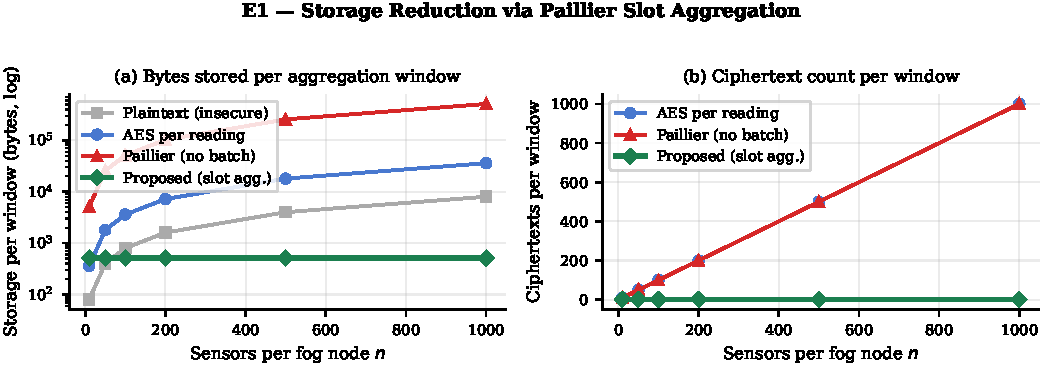
\includegraphics[width=1.0\linewidth]{figures/exp1_storage.pdf}
    \caption{E1: Storage comparison across schemes as a function of sensor count $n$. The upper panel shows total bytes; the lower panel shows ciphertext count. The proposed method stores one ciphertext per window for all $n$.}
    \label{fig:e1-storage}
    \end{figure}

    \subsection{E2: Aggregation Latency of the Python Prototype}
    \label{sec:eval-e2}

    \textbf{Objective.} Measure the end-to-end wall-clock latency of the proposed aggregation pipeline in the Python prototype and characterize per-component overhead.

    \textbf{Setup and baselines.} For $n\in\{10,50,100,200,500\}$ sensors per window, four pipelines are timed over three repetitions each: (i)~\emph{plaintext summation}, (ii)~\emph{AES-GCM encrypt-then-decrypt followed by sum}, (iii)~\emph{per-reading Paillier without aggregation}, and (iv)~the \emph{proposed pipeline} (SGX enclave AES-to-Paillier conversion, Paillier accumulation, KMM combine, and storage preparation). Median and standard deviation across repetitions are reported.

    \textbf{Results.} Fig.~\ref{fig:e2-latency} shows the latency results. Plaintext summation and AES-GCM encryption are negligible at all tested $n$ (under 1~ms and 4~ms, respectively). Both the per-reading Paillier baseline and the proposed pipeline substantially exceed the 500~ms window constraint at all values of $n$. At $n=100$, the proposed method requires a median of 7712~ms, of which 7528~ms is attributable to the SGX enclave phase (AES-to-Paillier conversion and accumulation), 73~ms to KMM combine, and 18~ms to storage preparation. This overhead reflects unoptimized Python big-integer arithmetic in the prototype and is not representative of deployment-target performance. The latency behavior of hardware-accelerated implementations is characterized separately in E7 (Section~\ref{sec:eval-e7}).

    \textbf{Key takeaway.} The Python prototype confirms that Paillier enclave conversion dominates end-to-end latency at all tested $n$. The 500~ms window constraint is not satisfied in the prototype; this is an implementation constraint, not a conceptual limitation of the scheme.

    \begin{figure}[htbp]
    \centering
    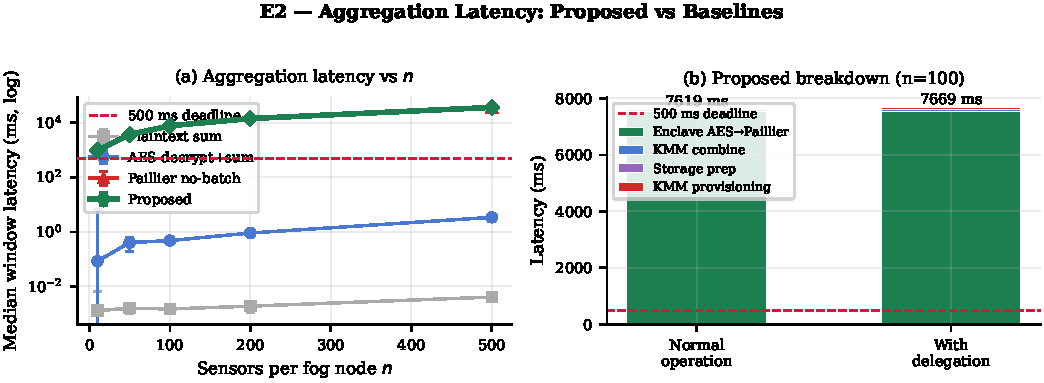
\includegraphics[width=1.0\linewidth]{figures/exp2_latency.pdf}
    \caption{E2: Aggregation latency vs sensor count $n$ for four pipeline configurations measured in the Python prototype. All Paillier-based configurations exceed the 500~ms window (dashed line) due to big-integer arithmetic overhead. The right panel shows the component breakdown of the proposed method at each $n$.}
    \label{fig:e2-latency}
    \end{figure}

    \subsection{E3: Slot Protocol Arithmetic Correctness Under Delegation}
    \label{sec:eval-e3}

    \textbf{Objective.} Verify that the Paillier slot protocol produces numerically correct aggregates when delegation occurs mid-window, for both single-source and multi-source delegation configurations.

    \subsubsection{E3a: Single-Source Delegation}
    \textbf{Setup.} A window of $n=100$ sensors is simulated with $k\in\{1,5,10,20,50\}$ sensors randomly delegated mid-window from primary node $F_1$ to backup node $F_4$. For each of 100 independent trials, the true scaled integer aggregate is computed directly from plaintext readings, and the output of the full slot protocol---AES-to-Paillier enclave conversion, Paillier accumulation with zero-fill for vacated slots, KMM combine, and decryption---is compared against it.

    \textbf{Results.} Across all values of $k$ and all 100 trials, the slot protocol produces zero scaled-integer error. A residual quantization error of approximately 0.045 (median absolute deviation from the true floating-point sum) is observed due to fixed-point integer encoding with $scale=1000$ and is consistent across all delegation counts. This is an inherent property of integer Paillier encoding rather than a protocol defect, and its magnitude is inversely proportional to the scaling factor.

    \subsubsection{E3b: Multi-Source Delegation}
    The protocol is further evaluated under simultaneous delegation from two sources ($F_1$ and $F_2$, each with 30 sensors) to a single backup node ($F_4$ with 30 own sensors), with 5 sensors per source delegated to $F_4$, for 100 independent trials. All 100 trials produce the correct scaled aggregate. The median quantization error is 0.041, consistent with the single-source case.

    \textbf{Key takeaway.} The Paillier slot protocol maintains aggregate correctness under mid-window delegation for both single and multi-source configurations across all 100 trials at every delegation count tested. These results constitute an arithmetic sanity check of the protocol implementation; they do not constitute a cryptographic proof of zero-fill ciphertext indistinguishability, which is argued analytically.

    \begin{figure}[htbp]
    \centering
    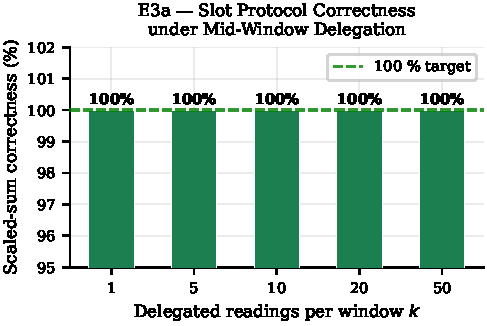
\includegraphics[width=1.0\linewidth]{figures/exp3a_correctness.pdf}
    \caption{E3a: Slot protocol correctness vs delegation count $k$ (100 trials, $n=100$ sensors). The upper panel shows 100\% accuracy at all $k$; the lower panel shows the quantization error due to fixed-point encoding with $scale=1000$.}
    \label{fig:e3a-correctness}
    \end{figure}

    \subsection{E4: KMM Window-Combine Overhead}
    \label{sec:eval-e4}

    \textbf{Objective.} Characterize the latency of the KMM homomorphic window-combine operation as the number of participating fog nodes $k$ increases from 1 to 100.

    \textbf{Setup.} For $k\in\{1,2,5,10,20,50,100\}$ fog aggregates, 30 repetitions of the \texttt{KMM.combine()} operation are timed. The measurement covers only the $k{-}1$ homomorphic additions over the received ciphertexts; ciphertext generation, zero encryption, and Paillier decryption are excluded. Each aggregate ciphertext is 512~bytes at the 2048-bit key size.

    \textbf{Results.} Fig.~\ref{fig:e4-kmm} shows that combine latency scales linearly with $k$. The operation requires 0.004~ms at $k=1$, 0.307~ms at $k=10$, 0.606~ms at $k=20$, and 3.24~ms at $k=100$. All values remain well within the 500~ms window budget.

    \textbf{Key takeaway.} The KMM combine step contributes negligible overhead across the full tested range of fog node counts. For a realistic deployment of up to $k=20$ fog nodes, the combine operation adds at most 0.606~ms to the window latency.

    \begin{figure}[htbp]
    \centering
    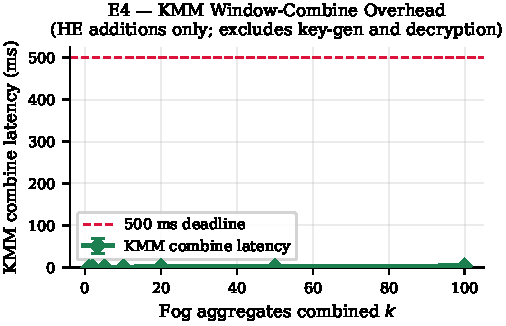
\includegraphics[width=1.0\linewidth]{figures/exp4_kmm_combine.pdf}
    \caption{E4: KMM window-combine latency vs number of fog aggregates $k$ (median over 30 repetitions; error bars show standard deviation). The dashed line marks 500~ms. The right panel shows total bytes received by the KMM at each $k$.}
    \label{fig:e4-kmm}
    \end{figure}

    \subsection{E5: Load Balancing Strategy Comparison}
    \label{sec:eval-e5}

    \textbf{Objective.} Compare the proposed $CapacityScore$-based delegation strategy against three heuristic baselines under a realistic dynamic load scenario incorporating node overload and failure events.

    \textbf{Setup and baselines.} A 20-window simulation with 100 tasks per window is run over five independent seeds. Tasks are partitioned as 70\% timeout-sensitive (TO) and 30\% latency-sensitive (LS). The window schedule introduces planned stress events: $F_2$ overload ($Workload=0.85>\tau$) during windows 6--10, $F_5$ failure during window 11 followed by gossip detection during windows 12--13 and recovery during windows 14--17, and a second $F_2$ overload ($Workload=0.90$) during windows 18--20. Four delegation strategies are compared: (1)~\emph{random} selection among available candidates; (2)~\emph{round-robin} cycling across candidates; (3)~\emph{threshold}, selecting the candidate with the minimum current workload; and (4)~\emph{capacity}, the proposed $CapacityScore$ strategy with task-adaptive weights.

    \textbf{Metrics.} Task completion rate, deadline satisfaction rate, re-delegation rate (fraction of tasks requiring a second delegation because the first target also became unavailable), and workload standard deviation across nodes are reported. Results are averaged over five seeds with 95\% confidence intervals.

    \textbf{Results.} Results are shown in Fig.~\ref{fig:e5-lb}. The capacity and threshold strategies both achieve 100\% task completion; random and round-robin achieve 88.56\% and 88.75\%, respectively, due to repeated selection of overloaded or failed targets. Deadline satisfaction rates are 93.03\% ($\pm$0.55\%) for capacity, 92.46\% ($\pm$0.66\%) for threshold, 81.48\% ($\pm$0.53\%) for round-robin, and 81.32\% ($\pm$1.69\%) for random. Both capacity and threshold produce 0\% re-delegation; random and round-robin each produce approximately 25\% re-delegation. Workload standard deviation is lowest under the capacity strategy (0.153) and highest under random (0.184), indicating more balanced distribution across nodes. A weight sensitivity analysis confirms that task completion remains at 100\% for all four weight configurations tested; deadline satisfaction degrades modestly (from 93\% to 92\%) only in the latency-heavy variant. These baselines are representative heuristics and are not claimed to represent state-of-the-art load balancing algorithms.

    \textbf{Key takeaway.} The $CapacityScore$ strategy achieves the highest deadline satisfaction rate and the lowest workload imbalance among the four strategies compared, while eliminating re-delegation. The threshold strategy is competitive in completion and re-delegation rate but produces higher workload imbalance.

    \begin{figure}[htbp]
    \centering
    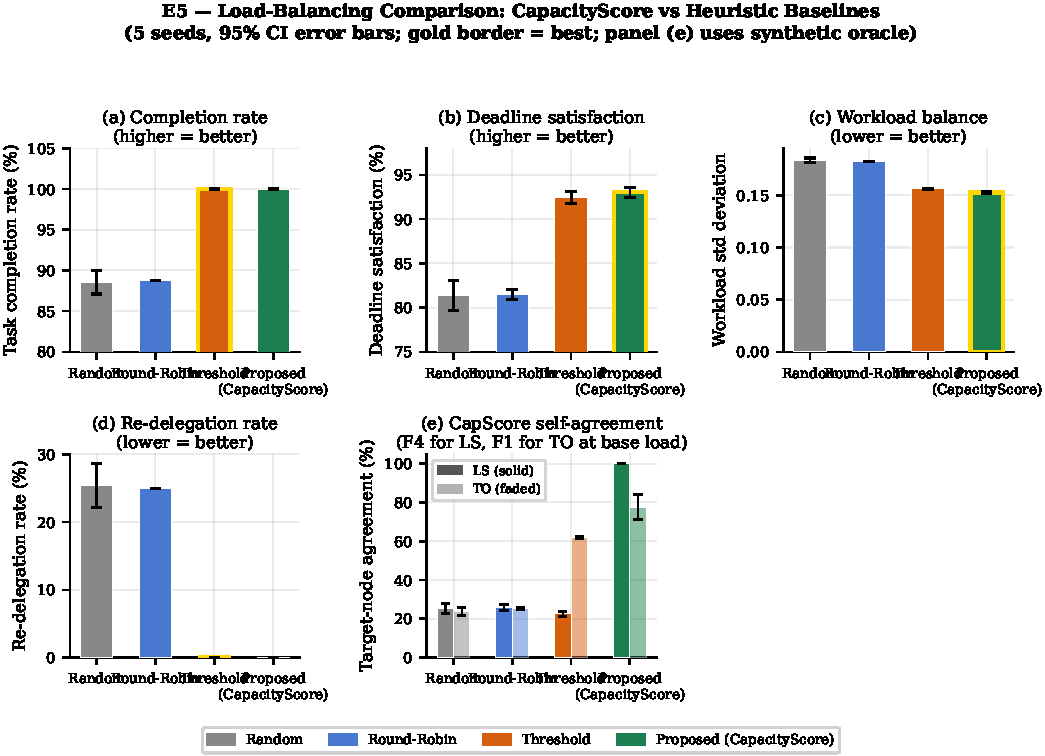
\includegraphics[width=1.0\linewidth]{figures/exp5_lb_comparison.pdf}
    \caption{E5: Load balancing comparison across four delegation strategies. Panels show task completion rate, deadline satisfaction rate, workload standard deviation, and re-delegation rate. Results are averaged over five seeds; error bars show 95\% CI.}
    \label{fig:e5-lb}
    \end{figure}

    \subsection{E6: Fault Detection and Recovery Analysis}
    \label{sec:eval-e6}

    \textbf{Objective.} Evaluate data loss rate and recovery latency of the proposed ACK+KMM fault recovery mechanism against five representative baselines across three failure timing scenarios.

    \textbf{Setup and baselines.} An analytical reading-loss model is evaluated over 30 simulation seeds and three failure scenarios: failure at the start of the observation window (\textit{fail\_0ms}), failure at 250~ms (\textit{mid\_window}), and failure at 450~ms (\textit{late\_window}). A total of 400 readings are generated per 500~ms window. Five baselines are evaluated: B1~gossip-based detection (failure declared after $r{=}3$ missed gossip rounds, detection latency $rT_g{=}1500\,\text{ms}$), B2~replication-based fault tolerance (each reading sent simultaneously to primary and backup), B3~checkpoint/restart (periodic checkpoint at 500~ms intervals, restore latency 500~ms), B4~multilayer detection (infrastructure and application layers combined, detection latency 500~ms), and B5~fog-cluster coordination (coordinator detects failure, selects replacement, and reroutes, total latency 750~ms). The proposed method uses sensor ACK timeout $T_{ack}{=}100\,\text{ms}$ followed by KMM key provisioning $T_{KMM}{=}50\,\text{ms}$, yielding a total recovery latency of 150~ms. All results are derived from the analytical model and should be interpreted as estimates relative to the modeled baselines rather than empirically measured end-to-end comparisons.

    \textbf{Results.} Fig.~\ref{fig:e6-fault} shows data loss rates and recovery latency across methods. In the worst-case scenario (failure at $t{=}0$), the proposed method loses approximately 6.5\% of readings (26 of 400 during the 150~ms recovery window), compared with 75\% for B1 gossip (1500~ms detection window), 25\% each for B3 checkpoint and B4 multilayer (500~ms windows), and approximately 38\% for B5 clustering (750~ms window). B2 replication achieves zero data loss at the cost of doubling message overhead. The proposed method incurs a message overhead of $1.055\times$ the baseline, attributable to per-reading ACK messages and two KMM provisioning messages per recovery event. Fig.~\ref{fig:e6-tradeoff} illustrates the data-loss versus message-overhead tradeoff space; the proposed method is nearest to the origin among single-mechanism approaches.

    \textbf{Key takeaway.} The proposed ACK+KMM mechanism reduces worst-case data loss from 75\% (gossip-only) to approximately 6.5\% while incurring only a 5.5\% increase in message overhead, representing a favorable tradeoff relative to all compared baselines except B2 replication, which achieves zero data loss at $2\times$ message cost.

    \begin{figure}[htbp]
    \centering
    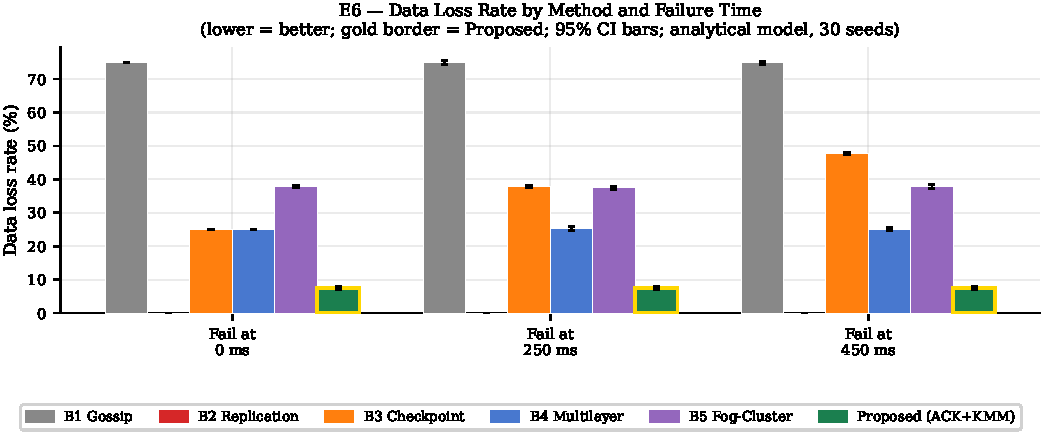
\includegraphics[width=1.0\linewidth]{figures/exp6_data_loss.pdf}
    \caption{E6: Data loss rate (upper) and recovery latency (lower) across six methods and three failure timing scenarios, averaged over 30 seeds with 95\% CI. Results are derived from an analytical reading-loss model.}
    \label{fig:e6-fault}
    \end{figure}

    \begin{figure}[htbp]
    \centering
    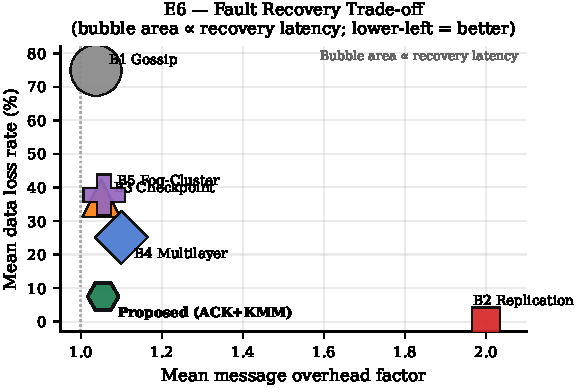
\includegraphics[width=1.0\linewidth]{figures/exp6_tradeoff.pdf}
    \caption{E6: Data loss vs message overhead tradeoff. Each marker represents one method; the proposed ACK+KMM method (green) is closest to the origin in loss--overhead space.}
    \label{fig:e6-tradeoff}
    \end{figure}

    \subsection{E7: End-to-End Pipeline Latency (Analytical Model)}
    \label{sec:eval-e7}

    \textbf{Objective.} Estimate end-to-end latency and per-window storage footprint of the proposed pipeline under hardware-accelerator assumptions and compare against three representative baselines across dynamic window conditions.

    \textbf{Setup and baselines.} The model uses hardware-target latency constants: sensor AES encryption (0.001~ms, hardware AES-NI), Paillier encryption per slot (3.8~ms, hardware-assisted co-processor), Paillier homomorphic addition (0.01~ms), KMM combine inside TEE (1.0~ms), storage preparation (5.0~ms), cloud upload (10.0~ms), and TEE key delegation round-trip (150.0~ms). For $n{=}100$ sensors, four methods are evaluated across the same 20-window schedule as E5: (i)~\emph{cloud-only} (raw sensor values uploaded directly, no fog processing), (ii)~\emph{fog plaintext} (fog accumulates an unencrypted sum; insecure lower bound), (iii)~\emph{Paillier-fog-convert} (per-reading Paillier encryption at the fog, no slot aggregation, one ciphertext per window sent to cloud), and (iv)~\emph{proposed}. These latency constants represent target deployment hardware and are explicitly \emph{not} comparable to the Python-measured E2 results reported in Section~\ref{sec:eval-e2}.

    \textbf{Results.} Fig.~\ref{fig:e7-pipeline} shows pipeline latency and per-window storage. Cloud-only and fog-plaintext complete in 40~ms and 13~ms, respectively; however, cloud-only stores 100 raw values per window (800~bytes) while fog-plaintext provides no data confidentiality. The Paillier-fog-convert baseline requires 393~ms and stores one 512-byte ciphertext per window, satisfying the 500~ms budget across all 20 windows. The proposed method requires 399~ms during non-delegation windows (12 of 20 windows) and 549~ms during delegation and failure-recovery windows (8 of 20 windows), where the additional 150~ms TEE key delegation step is active. Both the proposed method and the Paillier-fog-convert baseline store one aggregate per window, compared with 100 raw items per window for cloud-only.

    \textbf{Key takeaway.} Under hardware-target assumptions, the proposed method achieves the same aggregate storage efficiency as the Paillier-fog-convert baseline (one ciphertext per window) while additionally supporting delegation and fault recovery. The 500~ms budget is maintained in 12 of 20 windows; delegation and recovery windows incur an additional 150~ms, which is the cost of TEE key provisioning. The fog-plaintext baseline serves as a latency lower bound only and does not satisfy the confidentiality requirements of the proposed threat model.

    \begin{figure}[htbp]
    \centering
    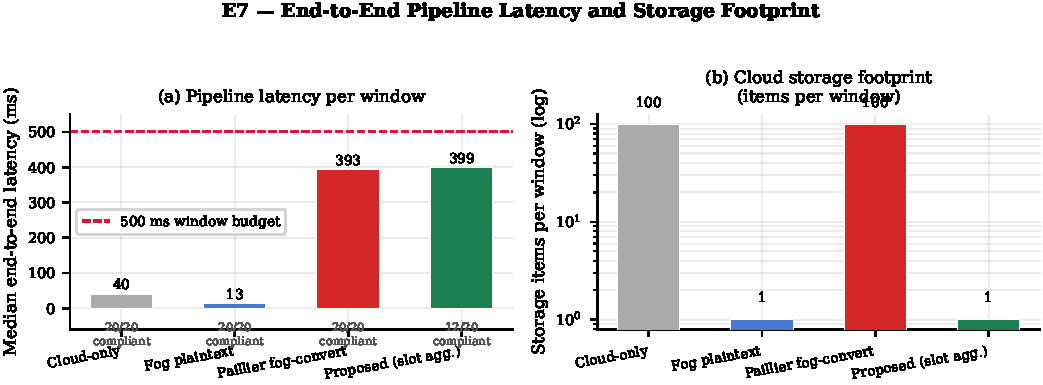
\includegraphics[width=1.0\linewidth]{figures/exp7_pipeline.pdf}
    \caption{E7: Analytical end-to-end pipeline latency (left) and per-window storage items (right) for four methods across 20 windows ($n{=}100$). The dashed line marks the 500~ms window budget. The proposed method exceeds this budget in 8 windows where TEE key delegation is active. \textbf{Note}: This is an analytical model using hardware-target constants; see Fig.~\ref{fig:e2-latency} for Python prototype measurements.}
    \label{fig:e7-pipeline}
    \end{figure}

    \subsection{E8: Key Exposure Blast Radius}
    \label{sec:eval-e8}

    \textbf{Objective.} Quantify the number of sensors whose decryption key is exposed under four threat scenarios, comparing a global shared AES key architecture with the proposed fog-scoped key design.

    \textbf{Setup.} The system consists of 100 sensors distributed evenly across five fog nodes (20 per node). Four compromise scenarios are evaluated using analytical exposure accounting: (i)~\emph{one fog node compromised} ($F_1$ enclave physically broken); (ii)~\emph{backup node compromised during active delegation} ($F_4$ enclave broken while holding a provisioned $k_{fogA}$ key); (iii)~\emph{KMM compromised}; and (iv)~\emph{host OS reads enclave memory} (under the standard SGX honest-but-curious threat model). These results represent analytical exposure counts and are not the product of a cryptographic attack simulation or SGX penetration test.

    \textbf{Results.} Fig.~\ref{fig:e8-blast} shows the results. In scenario~(i), a global key scheme exposes all 100 sensors while fog-scoped keys expose only the 20 sensors assigned to the compromised node, an 80\% reduction. In scenario~(ii), the backup node holds only $k_{fogA}$ provisioned for the current delegation epoch, exposing 40 sensors (20 from $F_1$ and 20 from $F_4$'s own group) versus all 100 under a global key, a 60\% reduction. In scenario~(iii), KMM compromise exposes all 100 sensors under both schemes, since the KMM is the trust anchor for both; no isolation benefit exists in this scenario. In scenario~(iv), the SGX assumption prevents host OS access to enclave memory in both schemes, so no sensors are exposed under either design.

    \textbf{Key takeaway.} Fog-scoped key isolation reduces sensor exposure by 60--80\% in single-node compromise scenarios relative to a global key design. The benefit does not extend to KMM compromise, which the threat model identifies as a critical single point of failure common to both schemes.

    \begin{figure}[htbp]
    \centering
    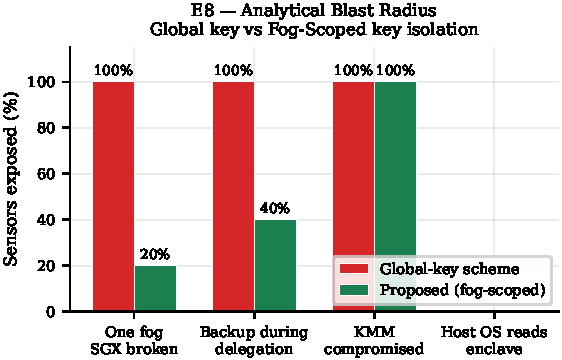
\includegraphics[width=1.0\linewidth]{figures/exp8_blast_radius.pdf}
    \caption{E8: Analytical key exposure comparison between a global AES key design and the proposed fog-scoped key design across four threat scenarios (100 sensors total, 20 per node). KMM compromise exposes all sensors under both schemes.}
    \label{fig:e8-blast}
    \end{figure}

    \section{Future Work}

    A limitation of the present work is that the $CapacityScore$ weights $(w_1, w_2, w_3)$ are fixed heuristics selected by task classification rather than learned from observed workload distributions. The sensitivity analysis in E5 demonstrates that deadline satisfaction degrades when weights are misconfigured relative to the actual task mix, motivating data-driven weight adaptation. An important direction for future work is to replace the static weight table with an online learning mechanism---such as a contextual bandit or lightweight reinforcement learning policy---that adjusts weights based on observed deadline miss rates and node utilization histories across aggregation windows. Additionally, the workload update model in E5 uses a formula-based service time derived from static node profiles rather than a principled queuing model; extending the simulation to a discrete-event framework with explicit queue dynamics (e.g., M/M/$c$ per node) would produce more accurate estimates of redelegation rates and deadline miss probabilities at larger scales. The present evaluation covers five fog nodes, 20 windows, and 100 tasks per window; characterizing system behavior under hundreds of nodes and high-variance arrival rates represents a necessary step toward deployment-scale validation. Furthermore, the current Paillier-based aggregation layer supports only additive operations---sum, mean, and weighted sum. Future work will extend the scheme to CKKS-based slot batching to support multiplicative aggregation functions such as variance, threshold count, and nonlinear statistics, and to provide approximate arithmetic over packed sensor vectors with formally bounded noise growth.

    The experimental evaluation rests on several simplifying assumptions that limit direct correspondence to real deployments. The SGX trusted execution environment is entirely simulated: \texttt{sgx\_enclave\_process} is implemented as an ordinary Python function performing AES decryption followed by Paillier encryption, with no actual enclave boundary, no sealing key derivation, and no remote attestation exchange. The KMM provisioning latency $T_{KMM}=50\,\text{ms}$ is a fixed design parameter rather than a measured quantity. Future work should implement the enclave layer using a real SGX SDK (e.g., Intel SGX SDK or Gramine) and validate provisioning latency on Skylake or Ice Lake class hardware. Similarly, the end-to-end pipeline latency in E7 is derived entirely from hardcoded hardware-target constants; these estimates should be replaced by measurements on physical fog hardware equipped with AES-NI and an SGX-capable processor. The CP-ABE cloud access control layer is fully specified in the scheme and notation but is absent from all experiment scripts: neither key generation, policy evaluation, nor attribute revocation overhead is measured. Integrating a standard CP-ABE implementation (e.g., Charm-Crypto) and characterizing its latency relative to the 500~ms aggregation window is an important open task. Finally, the multi-cluster Kubernetes analytics path described in the architecture has not been deployed or tested on any real cluster infrastructure; end-to-end validation of the authorized access path on a real Kubernetes environment would be required before the scheme can be considered production-ready.

    The fault tolerance evaluation in E6 is based on an analytical reading-loss model that counts sensor readings falling within a fixed failure-to-recovery time window under three predetermined failure timings. This model does not capture cascading failures, partial node degradation, network partition effects, or the interaction between simultaneous sensor ACK timeouts and the gossip convergence process. Future work should validate the proposed ACK+KMM recovery mechanism under realistic fault injection using network emulation tools such as tc-netem or a containerized testbed, and should extend the failure model to cover correlated multi-node failures and transient network outages. The gossip protocol parameters---fan-out $k{=}3$, miss threshold $r{=}3$, and gossip interval $T_g{=}500\,\text{ms}$---are fixed throughout the evaluation; the probabilistic detection model derived from the Poisson failure process provides a design criterion ($T_g \geq \ln(20)/(\mu r)$ for $\beta=0.95$), but adaptive parameter selection under varying failure rates $\mu$ has not been investigated. The KMM is currently modeled as a single trusted authority; future work may investigate threshold or multi-party key management constructions that distribute the trust anchor across a quorum of KMM instances, reducing the exposure when the KMM is compromised. Finally, the present scheme provides computational confidentiality under the IND-CPA assumption for Paillier and AES-GCM but does not address what an honest-but-curious cloud observer can infer from the sequence of decrypted aggregates over time. Investigating differential privacy mechanisms for the aggregate output, or bounding the statistical leakage of the published aggregate stream, remains an open problem for future work.

    \bibliographystyle{IEEEtran}
    \bibliography{references}

    \end{document}